{}\documentclass[letterpaper,
compress,
xcolor=x11names,
%draft,
]{beamer}
% Package imports
\usepackage{mathtools} % imports `amsmath'
\DeclareMathOperator{\sech}{sech}
\usepackage{amssymb}
\usepackage{fixltx2e}
\usepackage{lmodern}
\usepackage{movie15}
%\usepackage{media9}
\usepackage{microtype}
\usepackage{animate}
\usepackage{subcaption}
\captionsetup{compatibility=false}

% I just did this
\usepackage[english]{babel}
\usepackage[utf8]{inputenc}
\usepackage{amsmath}
\usepackage{graphicx}
\usepackage[colorinlistoftodos]{todonotes}
\usepackage{tikz}
\usetikzlibrary{tikzmark}
\usepackage{array}
\usepackage{layout}
\usepackage{multicol}
\usepackage{multirow}
\usepackage{booktabs}
%I just did this

% `beamer' configuration
\usefonttheme{professionalfonts}
\useoutertheme[subsection=false,]{miniframes}
\setbeamercolor*{alerted text}{fg=red}
\setbeamercolor*{example text}{fg=black}
\definecolor{CSU_green}{RGB}{30, 70, 43}
\definecolor{CSU_gold}{RGB}{200, 195, 114}
\setbeamercolor*{lower separation line head}{bg=CSU_gold}
\setbeamercolor*{section in head/foot}{fg=white,bg=CSU_green}
\setbeamercolor*{subsection in head/foot}{bg=white}
\setbeamercolor*{upper separation line head}{bg=CSU_gold}
\setbeamercolor*{page number in head/foot}{fg=CSU_green}
\setbeamercolor*{normal text}{fg=black,bg=white}
\setbeamercolor*{palette tertiary}{fg=black,bg=black!10}
\setbeamercolor*{palette quaternary}{fg=black,bg=black!10}
\setbeamercolor*{structure}{fg=black}
\setbeamerfont{frametitle}{shape=\scshape}
\setbeamerfont{institute}{shape=\scshape}
\setbeamerfont{section in head/foot}{shape=\scshape}
\setbeamerfont{subsection in head/foot}{shape=\scshape}
\setbeamertemplate{bibliography item}{}
\setbeamertemplate{itemize items}[ball]
\setbeamertemplate{navigation symbols}{}
\setbeamertemplate{footline}[frame number]
\usetikzlibrary{calc,arrows}
\graphicspath{{graphics/}{graphics/movies/}{graphics/images/}}
\usepackage{remreset}                  % hack to display beamer navigation
\makeatletter                          % circles even if not declaring
\@removefromreset{subsection}{section} % subsections
\makeatother                           % see: http://tex.stackexchange.com/a/2078
\setcounter{subsection}{1}             % see: https://bitbucket.org/rivanvx/beamer/issue/218

% `biblatex' configuration
\usepackage[backend=biber,
style=authortitle-comp,
]{biblatex}
\addbibresource{presentation.bib}

% `enumitem' configuration
\usepackage{enumitem}
\setlist[itemize,1]{label=\usebeamertemplate{itemize item}}
\setlist[itemize,2]{label=\usebeamertemplate{itemize subitem}}
\setlist[itemize,3]{label=\usebeamertemplate{itemize subsubitem}}
\DeclareMathOperator{\sinc}{sinc}


% `graphicx' configuration
\usepackage{graphicx}
\begin{document}
	\title{Ordinary Differential Equation Solvers}
	%\subtitle{MATH-151:  Mathematical Algorithms in Matlab}
	\author{MATH-151:  Mathematical Algorithms in Matlab}
	\date[202X]{October 16, 2023}
	\titlegraphic{
\includegraphics[height = 3cm]{CSU_Ram_Logo.jpg}}



%%%%%%%%%%%%%%%%%%%%%%%%%%%%%%%%%%%%%%%%%%%%%%%%%%%%%%

\begin{frame}
\titlepage
\end{frame}

%%%%%%%%%%%%%%%%%%%%%%%%%%%%%%%%%%%%%%%%%%%%%%%%%%%%%%

\begin{frame}{Embracing Change}
	\footnotesize
	\begin{itemize}
		\item In physical systems one of the most common things we want to answer is how things change, and further, how that change creates other change
		\begin{itemize}
			\item For example, me speeding up my legs accelerates me and changes the speed I'm walking. This changes how much where I am changes.
		\end{itemize}
		\item<2-> These relationships are almost always described as \textbf{differential equations}, which are equations that show how some quantity relates to its derivatives. We will see them in the form 
		\begin{equation*}
			y^{(m)}(t) = f(t,y,y',\dots,y^{(m-1)})
		\end{equation*}
		where $y^{(k)}$ is the kth derivative of the function $y(t)$
		\item<3-> We'll see some specific examples of these in a bit, but often to solve these we need to have some other information which come in two ``flavors"
		\begin{itemize}
			\item<4-> Sometimes we know a lot about where we start and want to know what happens afterwards, this is an \textbf{initial value problem} or IVP
			\item<5-> Other times we know what happens at two points and want to find what has happened in between, this is a \textbf{boundary value problem} or BVP
		\end{itemize}
	\end{itemize}
\end{frame}

%%%%%%%%%%%%%%%%%%%%%%%%%%%%%%%%%%%%%%%%%%%%%%%%%%%%%%%%%
\section{Initial Value Problems}

\begin{frame}{Starting on the Right Foot}
	\footnotesize
	\begin{itemize}
		\item We'll start with IVPs, in these cases we are given where our value of interest begins and use the differential equation to find how it changes.
		\item<2-> For example, we can write the equations for me starting to walk from a standstill as follows
		\begin{align*}
			&\frac{dv}{dt} = a(t) \\
			&\frac{dp}{dt} = v(t) \\
			&p(0) = 0,\hspace{0.25cm} v(0) = 0
		\end{align*}
		\item<3-> This is a \textbf{system of differential equations}, to know where I am we need to solve both of these together!
		\begin{itemize}
			\item Since we have two equations to solve, we have two pieces of information to start with
			\item Where was I standing and how fast was I traveling to begin with
		\end{itemize}
		\item<4-> The first equation tells me how my acceleration changes my speed, then once I know my speed I can see how that changes my position!
	\end{itemize}
\end{frame}

%%%%%%%%%%%%%%%%%%%%%%%%%%%%%%%%%%%%%%%%%%%%%%%%%%%%%%%%%%

\begin{frame}{Forward Euler Method}
	\footnotesize
	\begin{itemize}
		\item The most straightforward method for solving IVPs is to start at the beginning and ``march forward" by numerically integrating our equation to get the value at the next step
		\item<2-> What is the simplest way to do this? Since $y'= f(t,y)$ we can calculate $f(t,y_n)$ so we will use left rectangular rule to estimate the change!
		\item<2-> Doing this leaves us with the \textbf{forward Euler method}
		\begin{equation*}
			y_{n+1} = y_n + f(t,y_n)h
		\end{equation*}
		\item<3-> Let's try this with the IVP $y' = \frac{1}{2}y$ where $y(0) = 1$, with step size $h = 0.1$\\
		\begin{columns}
			\begin{column}{0.5\linewidth}
				\begin{equation*}
					y_{n+1} = y_n + h\frac{y_n}{2}
				\end{equation*}
				\begin{center}
					We can find the true solution is $y(t) = e^{\frac{t}{2}}$ \\
					\onslide<4->{Unfortunately, our approximation looks exponential, but it lags behind the \textcolor{red}{true solution}...}
				\end{center}
				
			\end{column}
			\begin{column}{0.5\linewidth}
				\begin{center}
					\only<3>{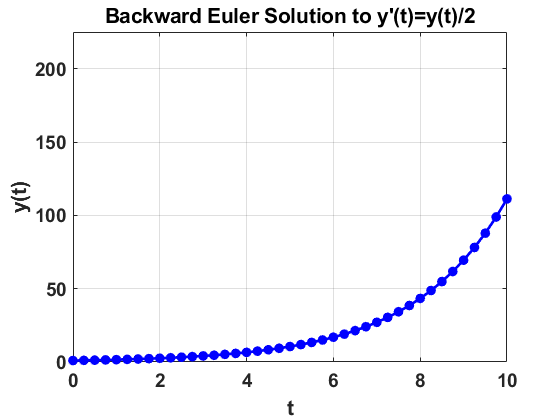
\includegraphics[height = 3cm]{Exp_Euler.png}}
					\only<4>{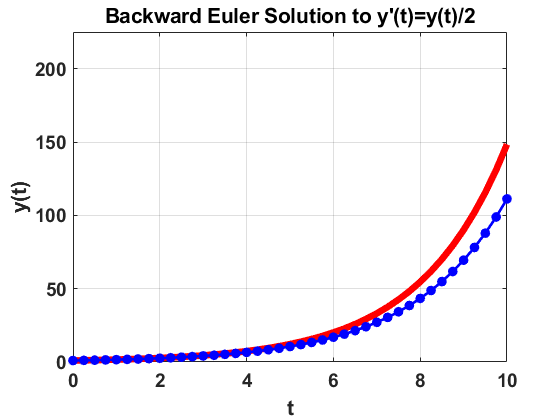
\includegraphics[height = 3cm]{Exp_Euler_wSln.png}}
				\end{center}
			\end{column}
		\end{columns}
	\end{itemize}
\end{frame}

%%%%%%%%%%%%%%%%%%%%%%%%%%%%%%%%%%%%%%%%%%%%%%%%%%%%%%%%%

\begin{frame}{Backward Euler Method}
	\footnotesize
	\begin{itemize}
		\item Forward Euler method is similar to our left rectangular rule, so maybe we might want to use right rectangular rule!
		\begin{equation*}
			y_{n+1} = y_n + f(t,y_{n+1})h
		\end{equation*}
		\item<2-> But wait! How can we calculate $f(t,y_{n+1})$ if we don't know $y_{n+1}$?
		\item<3-> We don't know it yet, but we can use our nonlinear solvers to solve $y_{n+1} - y_n - f(t,y_{n+1})h = 0$
		\item<3-> Solving these equations for each of our $y_n$ values gives us the \textbf{backward Euler method}
		\begin{center}
			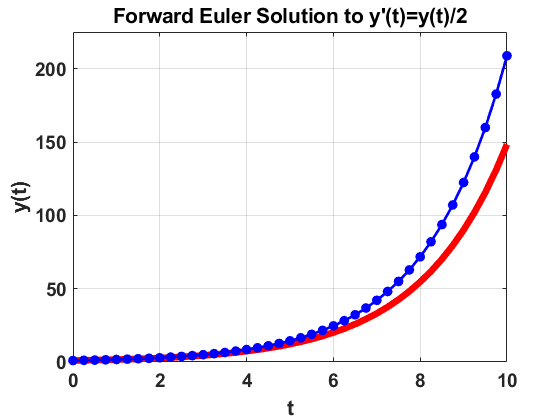
\includegraphics[height = 3cm]{Imp_Euler_w_Sln.png}
		\end{center}
		\item<4-> This still seems to be off, maybe we need to find a middle-ground between these two
	\end{itemize}
\end{frame}

%%%%%%%%%%%%%%%%%%%%%%%%%%%%%%%%%%%%%%%%%%%%%%%%%%%%%%%%%

\begin{frame}{Runge-Kutta Methods}
	\footnotesize
	\begin{itemize}
		\item Runge-Kutta methods are a class of ODE solver algorithms that find weighted averages of solutions
		\item<2-> The most commonly seen is the 4th-order Runge-Kutta algorithm, often called just RK4. It is similar to applying Simpson's rule to integrating our differential equation. We perform it as below
		\begin{align*}
			y_{n+1} &= y_n + \frac{h}{6}(k_1 + 2k_2 + 2k_3 + k_4) \\
			&k_1 = f(t_n, y_n) \\
			&k_2 = f(t_n + \frac{h}{2}, y_n + \frac{h}{2}k_1) \\
			&k_3 = f(t_n + \frac{h}{2}, y_n + \frac{h}{2}k_2) \\
			&k_4 = f(t_n + h, y_n + hk_3) 
		\end{align*}
		\item<3-> A quick way to think about it is that we keep trying to take half-steps forward and refining our guess of our slope
		\item<3-> It looks like a lot of work at first, but once you get comfortable it works very well!
	\end{itemize}
\end{frame}

%%%%%%%%%%%%%%%%%%%%%%%%%%%%%%%%%%%%%%%%%%%%%%%%%%%%%%%%%

\begin{frame}{Runge-Kutta Example Case}
	\footnotesize
	\begin{itemize}
		\item The general form may look scary, but lets look at it for our $y' = \frac{1}{2}y$ example, so $f(t,y) = \frac{1}{2}y$
		\onslide<2->{
		\begin{columns}
			\begin{column}{0.6\linewidth}
				\begin{align*}
					y_{n+1} &= y_n + \frac{h}{6}(k_1 + 2k_2 + 2k_3 + k_4) \\
					&k_1 = \frac{1}{2}y_n \\
					&k_2 = \frac{1}{2} (y_n + \frac{h}{2}k_1) \\
					&k_3 = \frac{1}{2} (y_n + \frac{h}{2}k_2)\\
					&k_4 = \frac{1}{2} (y_n + hk_3)
				\end{align*}
			\end{column}
			\begin{column}{0.4\linewidth}
				\begin{center}
					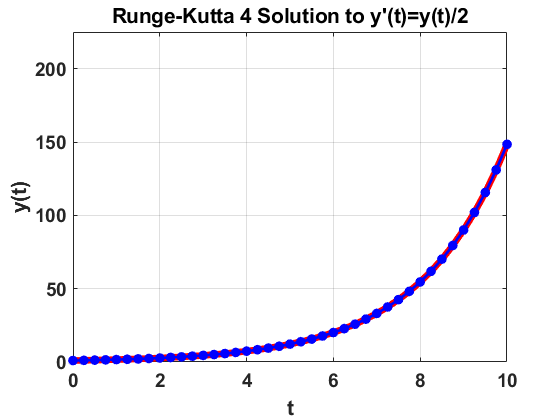
\includegraphics[height = 3.5cm]{RK4_wSln.png}
				\end{center}
			\end{column}
		\end{columns}	
		}	
		\item<3-> This is surprisingly straightforward to code up and it gives us VERY accurate solutions!
		\begin{itemize}
			\item Our maximum error in this example was 0.0014
		\end{itemize}
	\end{itemize}
\end{frame}

%%%%%%%%%%%%%%%%%%%%%%%%%%%%%%%%%%%%%%%%%%%%%%%%%%%%%%%%%
\section{Boundary Value Problems}

\begin{frame}{Setting Some Boundaries}
	\footnotesize
	\begin{itemize}
		\item Another major class of ODEs are \textbf{Boundary Value Problems} or BVPs, which are cases where we know the value of our function at two endpoints and want to find what the function does in between.
		\item<2-> Lets return to the problem of me walking around the room. Suppose instead I know I started here and ended up 
		\begin{align*}
			&\frac{dv}{dt} = a(t) \\
			&\frac{dp}{dt} = v(t) \\
			&p(0) = 0,\hspace{0.25cm} p(60) = 30
		\end{align*}
		\item<3-> Now this becomes less of a question of ``where did I go?" and more of a question of ``how did I get there?"
		\item<4-> These are more difficult to solve, we don't even have enough information to start ``marching forward" line we did for IVPs...
	\end{itemize}
\end{frame}

%%%%%%%%%%%%%%%%%%%%%%%%%%%%%%%%%%%%%%%%%%%%%%%%%%%%%%%%%

\begin{frame}{Shooting Method}
	\footnotesize
	\begin{itemize}
		\item ... but what if we just guess at what we think the initial conditions would be? We can then solve it like an IVP and see if we get to the right place
		\item<2-> If its wrong we can ``adjust our aim" and try again. We repeat this process using a nonlinear solver until we hit the target!
		\item<3-> Let's see it in practice. Suppose we have a soap bubble connected along two rings being pull apart. This bubble's shape will minimize the volume of a surface of revolution and satisfy the following BVP
		\begin{columns}
			\begin{column}{0.5\linewidth}
				\begin{align*}
					&\frac{du'}{dx}(x) = \frac{1 + u'(x)^2}{u(x)} \\
					&\frac{du}{dx}(x) = u'(x) \\
					&u(0) = 10, \hspace{0.1cm} u(10) = 7
				\end{align*} 
			\end{column}
			\begin{column}{0.5\linewidth} \\
				\only<4>{\underline{Lets aim flat} \\ 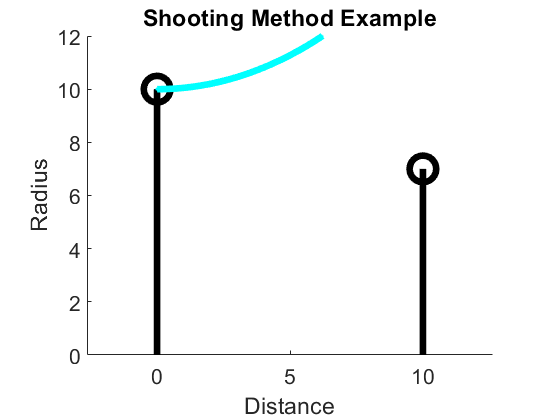
\includegraphics[width=0.75\linewidth]{Shooting_1.png}}
				\only<5>{\underline{Too high, lets aim lower} \\ 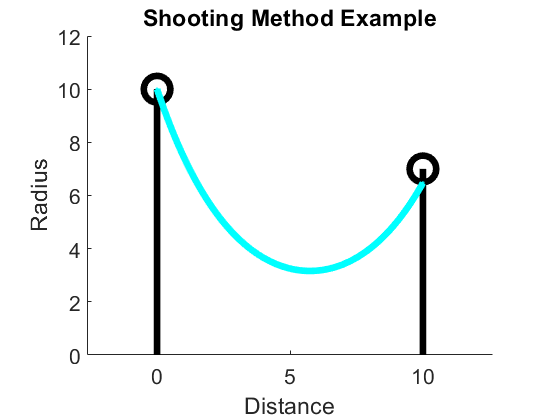
\includegraphics[width=0.75\linewidth]{Shooting_2.png}}
				\only<6>{\underline{We keep adjusting until} \\ 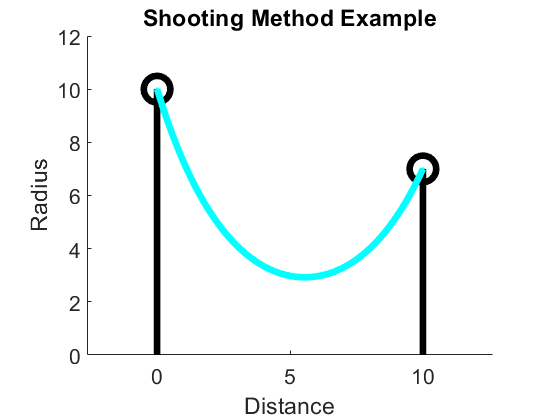
\includegraphics[width=0.75\linewidth]{Shooting_final.png}}
			\end{column}
		\end{columns}
	\end{itemize}

\end{frame}

%%%%%%%%%%%%%%%%%%%%%%%%%%%%%%%%%%%%%%%%%%%%%%%%%%%%%%%%%
\end{document}